\documentclass[12pt]{article}\usepackage[]{graphicx}\usepackage[]{color}
%% maxwidth is the original width if it is less than linewidth
%% otherwise use linewidth (to make sure the graphics do not exceed the margin)
\makeatletter
\def\maxwidth{ %
  \ifdim\Gin@nat@width>\linewidth
    \linewidth
  \else
    \Gin@nat@width
  \fi
}
\makeatother

\definecolor{fgcolor}{rgb}{0.345, 0.345, 0.345}
\newcommand{\hlnum}[1]{\textcolor[rgb]{0.686,0.059,0.569}{#1}}%
\newcommand{\hlstr}[1]{\textcolor[rgb]{0.192,0.494,0.8}{#1}}%
\newcommand{\hlcom}[1]{\textcolor[rgb]{0.678,0.584,0.686}{\textit{#1}}}%
\newcommand{\hlopt}[1]{\textcolor[rgb]{0,0,0}{#1}}%
\newcommand{\hlstd}[1]{\textcolor[rgb]{0.345,0.345,0.345}{#1}}%
\newcommand{\hlkwa}[1]{\textcolor[rgb]{0.161,0.373,0.58}{\textbf{#1}}}%
\newcommand{\hlkwb}[1]{\textcolor[rgb]{0.69,0.353,0.396}{#1}}%
\newcommand{\hlkwc}[1]{\textcolor[rgb]{0.333,0.667,0.333}{#1}}%
\newcommand{\hlkwd}[1]{\textcolor[rgb]{0.737,0.353,0.396}{\textbf{#1}}}%
\let\hlipl\hlkwb

\usepackage{framed}
\makeatletter
\newenvironment{kframe}{%
 \def\at@end@of@kframe{}%
 \ifinner\ifhmode%
  \def\at@end@of@kframe{\end{minipage}}%
  \begin{minipage}{\columnwidth}%
 \fi\fi%
 \def\FrameCommand##1{\hskip\@totalleftmargin \hskip-\fboxsep
 \colorbox{shadecolor}{##1}\hskip-\fboxsep
     % There is no \\@totalrightmargin, so:
     \hskip-\linewidth \hskip-\@totalleftmargin \hskip\columnwidth}%
 \MakeFramed {\advance\hsize-\width
   \@totalleftmargin\z@ \linewidth\hsize
   \@setminipage}}%
 {\par\unskip\endMakeFramed%
 \at@end@of@kframe}
\makeatother

\definecolor{shadecolor}{rgb}{.97, .97, .97}
\definecolor{messagecolor}{rgb}{0, 0, 0}
\definecolor{warningcolor}{rgb}{1, 0, 1}
\definecolor{errorcolor}{rgb}{1, 0, 0}
\newenvironment{knitrout}{}{} % an empty environment to be redefined in TeX

\usepackage{alltt}
\usepackage{amsmath}
\usepackage{amssymb}
\usepackage{graphicx}
\usepackage{fullpage}
\usepackage{setspace}
\usepackage{hyperref}
\usepackage{color}
\onehalfspacing
\IfFileExists{upquote.sty}{\usepackage{upquote}}{}
\begin{document}

\title{Pol Sci 630: Problem Set 5 - Regression Model Interpretation - Solutions}

\author{Prepared by: Jan Vogler (\href{mailto:jan.vogler@duke.edu}{jan.vogler@duke.edu})}

\date{Grading Due Date: Friday, October 7th, 1.40 PM (Beginning of Lab)}
 
\maketitle



\textbf{\color{red} Insert your comments on the assignment that you are grading above the solution in bold and red text. For example write: ``GRADER COMMENT: everything is correct!" Also briefly point out which, if any, problems were not solved correctly and what the mistake was. See below for more examples.}

\bigskip

\textbf{In order to make your text bold and red, you need to insert the following line at the beginning of the document:}

\begin{verbatim} \usepackage{color} \end{verbatim}

\\ \textbf{and the following lines above the solution of the specific task:}

\begin{verbatim} \textbf{\color{red} GRADER COMMENT: everything is correct!} \end{verbatim}



\pagebreak

\section*{R Programming}

\subsection*{Problem 1}

\begin{knitrout}
\definecolor{shadecolor}{rgb}{0.969, 0.969, 0.969}\color{fgcolor}\begin{kframe}
\begin{alltt}
\hlcom{### a}

\hlkwd{data}\hlstd{(swiss)}
\hlkwd{summary}\hlstd{(swiss)}
\end{alltt}
\begin{verbatim}
##    Fertility      Agriculture     Examination      Education    
##  Min.   :35.00   Min.   : 1.20   Min.   : 3.00   Min.   : 1.00  
##  1st Qu.:64.70   1st Qu.:35.90   1st Qu.:12.00   1st Qu.: 6.00  
##  Median :70.40   Median :54.10   Median :16.00   Median : 8.00  
##  Mean   :70.14   Mean   :50.66   Mean   :16.49   Mean   :10.98  
##  3rd Qu.:78.45   3rd Qu.:67.65   3rd Qu.:22.00   3rd Qu.:12.00  
##  Max.   :92.50   Max.   :89.70   Max.   :37.00   Max.   :53.00  
##     Catholic       Infant.Mortality
##  Min.   :  2.150   Min.   :10.80   
##  1st Qu.:  5.195   1st Qu.:18.15   
##  Median : 15.140   Median :20.00   
##  Mean   : 41.144   Mean   :19.94   
##  3rd Qu.: 93.125   3rd Qu.:21.70   
##  Max.   :100.000   Max.   :26.60
\end{verbatim}
\begin{alltt}
\hlcom{### b}

\hlstd{lm1} \hlkwb{=} \hlkwd{lm}\hlstd{(Education} \hlopt{~} \hlstd{Fertility} \hlopt{+} \hlstd{Agriculture} \hlopt{+} \hlstd{Examination} \hlopt{+} \hlstd{Catholic} \hlopt{+} \hlstd{Infant.Mortality,}
    \hlkwc{data} \hlstd{= swiss)}

\hlkwd{summary}\hlstd{(lm1)}
\end{alltt}
\begin{verbatim}
## 
## Call:
## lm(formula = Education ~ Fertility + Agriculture + Examination + 
##     Catholic + Infant.Mortality, data = swiss)
## 
## Residuals:
##      Min       1Q   Median       3Q      Max 
## -11.3949  -2.3716  -0.2856   2.8108  11.2985 
## 
## Coefficients:
##                  Estimate Std. Error t value Pr(>|t|)    
## (Intercept)      32.74414    8.87888   3.688 0.000657 ***
## Fertility        -0.40851    0.08585  -4.758 2.43e-05 ***
## Agriculture      -0.16242    0.04488  -3.619 0.000804 ***
## Examination       0.41980    0.16339   2.569 0.013922 *  
## Catholic          0.10023    0.02150   4.663 3.29e-05 ***
## Infant.Mortality  0.20408    0.28390   0.719 0.476305    
## ---
## Signif. codes:  0 '***' 0.001 '**' 0.01 '*' 0.05 '.' 0.1 ' ' 1
## 
## Residual standard error: 4.907 on 41 degrees of freedom
## Multiple R-squared:  0.7678,	Adjusted R-squared:  0.7395 
## F-statistic: 27.12 on 5 and 41 DF,  p-value: 5.223e-12
\end{verbatim}
\end{kframe}
\end{knitrout}

\subparagraph{c)} \textbf{In order to get full points on this problem, you need an interpretation for each of the 5 variables.}

The interpretation would look like this for \textit{Fertility}:

There is a negative linear relationship between \textit{Fertility} and \textit{Education}. For a 1-point increase in Fertility, we expect a 0.41-point decrease in Education, holding all other variables constant. The t-value is -4.758. This t-value implies a p-value of $2.43*10^{-5}$. This $p < 0.001$ corresponds to a type-1 error rate of $\alpha < 0.001$, meaning that the statistical relationship is significant at all common levels of statistical significance.

The other variables are interpreted accordingly. \textit{Agriculture} and \textit{Catholic} are significant at all common levels of statistical significance as well. Please note that \textit{Examination} is significant at a level of $p < 0.05$ ($\alpha < 0.05$) and \textit{Infant.Mortality} is not significant at common levels of statistical significance.

The $R^2$ statistic shows us that our model explains 76.78 percent (multiple $R^2$) or 73.95 percent (adjusted $R^2$) of the variation in the dependent variabl. The adjusted $R^2$ is smaller because we are penalized for every variable that is introduced into our model.

The F-statistic shows us that the joint statistical significance of the variables in our model when predicting levels of \textit{Education} is high. With a p-value of $p < 0.001$, our model has an overall predictive capability that is significant at all common levels of statistical significance.

\begin{table}[!htbp] \centering 
  \caption{Regression: Education} 
  \label{} 
\begin{tabular}{@{\extracolsep{5pt}}lc} 
\\[-1.8ex]\hline 
\hline \\[-1.8ex] 
 & \multicolumn{1}{c}{\textit{Dependent variable:}} \\ 
\cline{2-2} 
\\[-1.8ex] & Education \\ 
\hline \\[-1.8ex] 
 Fertility & $-$0.409$^{***}$ \\ 
  & (0.086) \\ 
  Agriculture & $-$0.162$^{***}$ \\ 
  & (0.045) \\ 
  Examination & 0.420$^{**}$ \\ 
  & (0.163) \\ 
  Catholic & 0.100$^{***}$ \\ 
  & (0.021) \\ 
  Infant.Mortality & 0.204 \\ 
  & (0.284) \\ 
  Constant & 32.744$^{***}$ \\ 
  & (8.879) \\ 
 \hline \\[-1.8ex] 
Observations & 47 \\ 
R$^{2}$ & 0.768 \\ 
Adjusted R$^{2}$ & 0.740 \\ 
Residual Std. Error & 4.907 (df = 41) \\ 
F Statistic & 27.121$^{***}$ (df = 5; 41) \\ 
\hline 
\hline \\[-1.8ex] 
\textit{Note:}  & \multicolumn{1}{r}{$^{*}$p$<$0.1; $^{**}$p$<$0.05; $^{***}$p$<$0.01} \\ 
\end{tabular} 
\end{table}

\subsection*{Problem 2}

\paragraph{a)} In this task you have to formulate a hypothesis regarding the relationship of one variable and the vote share of party A. For example, you could claim that a higher level of expenditures of party A lead to a higher vote share because with more resources at its disposal, party A can air more advertisements, reach more voters, and mobilize more of its supporters.

Hypothesis: For an increase in the expenditures of party A, we expect an increase in the vote share of party A. (Regardless of which variable you choose, your hypothesis should look similar to this one.)

\paragraph{b)} 

\begin{knitrout}
\definecolor{shadecolor}{rgb}{0.969, 0.969, 0.969}\color{fgcolor}\begin{kframe}
\begin{alltt}
\hlcom{### b}
\hlkwd{library}\hlstd{(foreign)}
\hlstd{vote1} \hlkwb{=} \hlkwd{read.dta}\hlstd{(}\hlstr{"VOTE1.dta"}\hlstd{)}
\hlkwd{summary}\hlstd{(vote1)}
\end{alltt}
\begin{verbatim}
##     state              district          democA           voteA     
##  Length:173         Min.   : 1.000   Min.   :0.0000   Min.   :16.0  
##  Class :character   1st Qu.: 3.000   1st Qu.:0.0000   1st Qu.:36.0  
##  Mode  :character   Median : 6.000   Median :1.0000   Median :50.0  
##                     Mean   : 8.838   Mean   :0.5549   Mean   :50.5  
##                     3rd Qu.:11.000   3rd Qu.:1.0000   3rd Qu.:65.0  
##                     Max.   :42.000   Max.   :1.0000   Max.   :84.0  
##     expendA            expendB           prtystrA        lexpendA     
##  Min.   :   0.302   Min.   :   0.93   Min.   :22.00   Min.   :-1.197  
##  1st Qu.:  81.634   1st Qu.:  60.05   1st Qu.:44.00   1st Qu.: 4.402  
##  Median : 242.782   Median : 221.53   Median :50.00   Median : 5.492  
##  Mean   : 310.611   Mean   : 305.09   Mean   :49.76   Mean   : 5.026  
##  3rd Qu.: 457.410   3rd Qu.: 450.72   3rd Qu.:56.00   3rd Qu.: 6.126  
##  Max.   :1470.674   Max.   :1548.19   Max.   :71.00   Max.   : 7.293  
##     lexpendB            shareA        
##  Min.   :-0.07257   Min.   : 0.09464  
##  1st Qu.: 4.09524   1st Qu.:18.86800  
##  Median : 5.40056   Median :50.84990  
##  Mean   : 4.94437   Mean   :51.07654  
##  3rd Qu.: 6.11084   3rd Qu.:84.25510  
##  Max.   : 7.34484   Max.   :99.49500
\end{verbatim}
\begin{alltt}
\hlstd{lm_vote} \hlkwb{=} \hlkwd{lm}\hlstd{(voteA} \hlopt{~} \hlstd{expendA} \hlopt{+} \hlstd{expendB} \hlopt{+} \hlstd{prtystrA,} \hlkwc{data} \hlstd{= vote1)}
\hlkwd{summary}\hlstd{(lm_vote)}
\end{alltt}
\begin{verbatim}
## 
## Call:
## lm(formula = voteA ~ expendA + expendB + prtystrA, data = vote1)
## 
## Residuals:
##     Min      1Q  Median      3Q     Max 
## -26.661  -8.385   0.362   8.536  30.814 
## 
## Coefficients:
##              Estimate Std. Error t value Pr(>|t|)    
## (Intercept) 33.267190   4.416784   7.532 2.87e-12 ***
## expendA      0.034924   0.003369  10.365  < 2e-16 ***
## expendB     -0.034924   0.003001 -11.636  < 2e-16 ***
## prtystrA     0.342514   0.087952   3.894 0.000142 ***
## ---
## Signif. codes:  0 '***' 0.001 '**' 0.01 '*' 0.05 '.' 0.1 ' ' 1
## 
## Residual standard error: 11.12 on 169 degrees of freedom
## Multiple R-squared:  0.5687,	Adjusted R-squared:  0.561 
## F-statistic: 74.27 on 3 and 169 DF,  p-value: < 2.2e-16
\end{verbatim}
\end{kframe}
\end{knitrout}

Let us interpret our findings for the hypothesis above:

\textit{expendA}: For a 1-point increase in the expenditures of party A, we expect a 0.0349 (0.03) increase in the the vote share of party of party A, holding all other variables constant. The associated p-value of $p < 0.001$ means that this relationship is statistically significant at all common levels of statistical significance. This means that there is strong support  for the hypothesis that increases in the expenditures of A increase its vote share.

The $R^2$ statistic shows us that our model explains 56.87 percent (multiple $R^2$) or 56.1 percent (adjusted $R^2$) of the variation in the dependent variable. The adjusted $R^2$ is smaller because we are penalized for every variable that is introduced into our model.

The F-statistic shows us that the joint statistical significance of the variables in our model when predicting levels of FDI inflows is high. With a p-value of $p < 0.001$, our model has an overall predictive capability that is significant at all common levels of statistical significance.

\paragraph{c)} 

\begin{table}[!htbp] \centering 
  \caption{} 
  \label{} 
\begin{tabular}{@{\extracolsep{5pt}}lc} 
\\[-1.8ex]\hline 
\hline \\[-1.8ex] 
 & \multicolumn{1}{c}{\textit{Dependent variable:}} \\ 
\cline{2-2} 
\\[-1.8ex] & voteA \\ 
\hline \\[-1.8ex] 
 expendA & 0.035$^{***}$ \\ 
  & (0.003) \\ 
  & \\ 
 expendB & $-$0.035$^{***}$ \\ 
  & (0.003) \\ 
  & \\ 
 prtystrA & 0.343$^{***}$ \\ 
  & (0.088) \\ 
  & \\ 
 Constant & 33.267$^{***}$ \\ 
  & (4.417) \\ 
  & \\ 
\hline \\[-1.8ex] 
Observations & 173 \\ 
R$^{2}$ & 0.569 \\ 
Adjusted R$^{2}$ & 0.561 \\ 
Residual Std. Error & 11.121 (df = 169) \\ 
F Statistic & 74.267$^{***}$ (df = 3; 169) \\ 
\hline 
\hline \\[-1.8ex] 
\textit{Note:}  & \multicolumn{1}{r}{$^{*}$p$<$0.1; $^{**}$p$<$0.05; $^{***}$p$<$0.01} \\ 
\end{tabular} 
\end{table} 

\paragraph{d)}

Finally, we show the effect graphically:

\begin{knitrout}
\definecolor{shadecolor}{rgb}{0.969, 0.969, 0.969}\color{fgcolor}\begin{kframe}
\begin{alltt}
\hlcom{### We create a new dataframe with the average values for every variable and}
\hlcom{### vary Polity IV}
\hlstd{nd} \hlkwb{<-} \hlkwd{data.frame}\hlstd{(}\hlkwc{expendA} \hlstd{=} \hlkwd{seq}\hlstd{(}\hlkwd{min}\hlstd{(vote1}\hlopt{$}\hlstd{expendA),} \hlkwd{max}\hlstd{(vote1}\hlopt{$}\hlstd{expendA),} \hlkwc{length.out} \hlstd{=} \hlnum{11}\hlstd{),}
    \hlkwc{expendB} \hlstd{=} \hlkwd{rep}\hlstd{(}\hlkwd{mean}\hlstd{(vote1}\hlopt{$}\hlstd{expendB),} \hlnum{11}\hlstd{),} \hlkwc{prtystrA} \hlstd{=} \hlkwd{rep}\hlstd{(}\hlkwd{mean}\hlstd{(vote1}\hlopt{$}\hlstd{prtystrA),}
        \hlnum{11}\hlstd{))}

\hlstd{pred.p1} \hlkwb{<-} \hlkwd{predict}\hlstd{(lm_vote,} \hlkwc{type} \hlstd{=} \hlstr{"response"}\hlstd{,} \hlkwc{se.fit} \hlstd{=} \hlnum{TRUE}\hlstd{,} \hlkwc{newdata} \hlstd{= nd)}

\hlstd{pred.table} \hlkwb{<-} \hlkwd{cbind}\hlstd{(pred.p1}\hlopt{$}\hlstd{fit, pred.p1}\hlopt{$}\hlstd{se.fit)}

\hlstd{fit} \hlkwb{<-} \hlstd{pred.p1}\hlopt{$}\hlstd{fit}
\hlstd{low} \hlkwb{<-} \hlstd{pred.p1}\hlopt{$}\hlstd{fit} \hlopt{-} \hlnum{2} \hlopt{*} \hlstd{pred.p1}\hlopt{$}\hlstd{se.fit}
\hlstd{high} \hlkwb{<-} \hlstd{pred.p1}\hlopt{$}\hlstd{fit} \hlopt{+} \hlnum{2} \hlopt{*} \hlstd{pred.p1}\hlopt{$}\hlstd{se.fit}
\hlstd{cis} \hlkwb{<-} \hlkwd{cbind}\hlstd{(fit, low, high)}

\hlstd{cis}  \hlcom{### To extract the values}
\end{alltt}
\begin{verbatim}
##         fit      low     high
## 1  39.66551 36.97617 42.35485
## 2  44.80071 42.78322 46.81819
## 3  49.93590 48.24133 51.63048
## 4  55.07110 53.16411 56.97809
## 5  60.20630 57.68334 62.72926
## 6  65.34150 62.01619 68.66680
## 7  70.47669 66.26793 74.68546
## 8  75.61189 70.48028 80.74350
## 9  80.74709 74.67117 86.82301
## 10 85.88229 78.84923 92.91534
## 11 91.01748 83.01907 99.01589
\end{verbatim}
\begin{alltt}
\hlkwd{plot}\hlstd{(pred.p1}\hlopt{$}\hlstd{fit,} \hlkwc{type} \hlstd{=} \hlstr{"l"}\hlstd{,} \hlkwc{ylim} \hlstd{=} \hlkwd{c}\hlstd{(}\hlnum{35}\hlstd{,} \hlnum{100}\hlstd{),} \hlkwc{main} \hlstd{=} \hlstr{"Incumbent expenditures and vote share"}\hlstd{,}
    \hlkwc{xlab} \hlstd{=} \hlstr{"Incumbent expenditures"}\hlstd{,} \hlkwc{ylab} \hlstd{=} \hlstr{"Vote share"}\hlstd{,} \hlkwc{axes} \hlstd{=} \hlnum{FALSE}\hlstd{)}
\hlkwd{axis}\hlstd{(}\hlnum{1}\hlstd{,} \hlkwc{at} \hlstd{=} \hlkwd{seq}\hlstd{(}\hlnum{1}\hlstd{,} \hlnum{11}\hlstd{),} \hlkwc{labels} \hlstd{=} \hlkwd{round}\hlstd{(}\hlkwd{seq}\hlstd{(}\hlkwd{min}\hlstd{(vote1}\hlopt{$}\hlstd{expendA),} \hlkwd{max}\hlstd{(vote1}\hlopt{$}\hlstd{expendA),}
    \hlkwc{length.out} \hlstd{=} \hlnum{11}\hlstd{)))}
\hlkwd{axis}\hlstd{(}\hlnum{2}\hlstd{,} \hlkwc{at} \hlstd{=} \hlkwd{seq}\hlstd{(}\hlnum{35}\hlstd{,} \hlnum{100}\hlstd{,} \hlkwc{by} \hlstd{=} \hlnum{5}\hlstd{),} \hlkwc{labels} \hlstd{=} \hlkwd{seq}\hlstd{(}\hlnum{35}\hlstd{,} \hlnum{100}\hlstd{,} \hlkwc{by} \hlstd{=} \hlnum{5}\hlstd{))}
\hlkwd{matlines}\hlstd{(cis[,} \hlkwd{c}\hlstd{(}\hlnum{2}\hlstd{,} \hlnum{3}\hlstd{)],} \hlkwc{lty} \hlstd{=} \hlnum{2}\hlstd{,} \hlkwc{col} \hlstd{=} \hlstr{"black"}\hlstd{)}
\end{alltt}
\end{kframe}
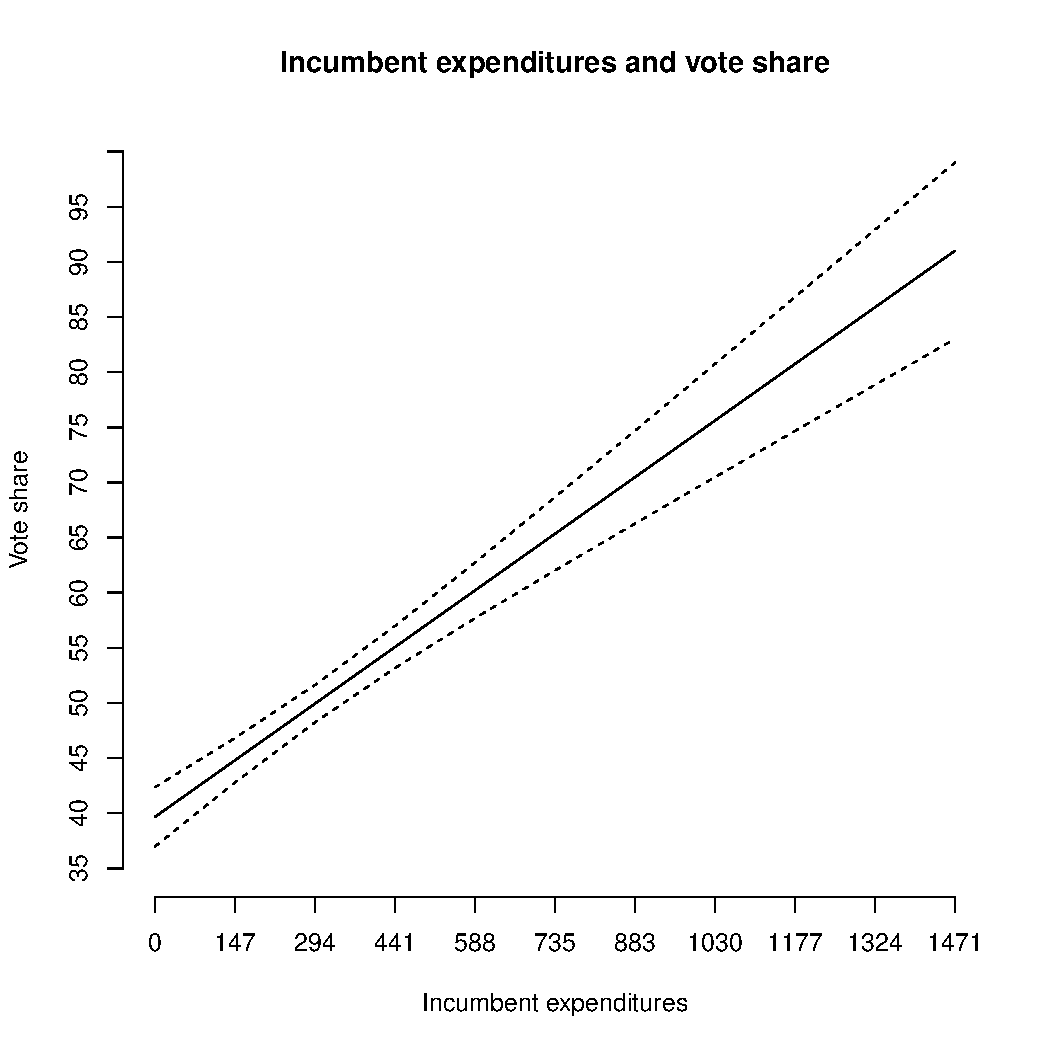
\includegraphics[width=\maxwidth]{figure/unnamed-chunk-3-1} 

\end{knitrout}



\section*{Linear Regression Models Interpretation Questions}

\subsection*{Problem 3}

\paragraph*{a)} If we do not include polynomials of higher order, OLS regression can adequately model only \textbf{linear} relationships between one dependent variable (response variable) and one or multiple independent variables (predictor variables).

The reason for why we can only model linear relationships is that our model assumes that for every independent variable there is only a single slope coefficient that is constant for all values of that independent variable. In other words, it assumes direct proportionality. The additional inclusion of polynomials of higher order would allow us to have different slopes at different values of the independent variable.

\paragraph*{b)} OLS regression does not per se tell us anything about causality. OLS regression primarily measures linear relationships between two variables and can give us an answer to the question how to variables are correlated with each other. However, without a strong theory, OLS does not allow us to make statements regarding causality.

There are several reasons for this. First, there could be reverse causality, meaning that the response variable in our model has a causal effect on the predictor variable. Second, there could be endogeneity, meaning that there is mutual causal influence of response and predictor variables. Third, there could be omitted variable bias, meaning that a third variable influences both the predictor and the response variable. Fourth, there could be ``parallel trends", meaning that although two variables have no relationship to each other, they only move simultaneously. For example, two variables could both increase over time for completeley different reasons, potentially giving the wrong impression that they are causally connected. These are the four main reasons why we should not per se view the results of a linear regression as reflecting causality.

\paragraph*{c)} The Residual Sum of Squares (RSS) can be found through the following calculation involving the Root Mean Squared Error (RMSE):

\bigskip

RSS = $(RMSE^2)*(Degrees\ of \ Freedom)$

\bigskip

Furthermore, given that we know $R^2$, once we know the RSS, we can use the fact that $R^2 = 1 - \dfrac{RSS}{TSS}$ to find that:

\bigskip

$\dfrac{1 - R^2}{RSS} = \dfrac{1}{TSS}$ \rightarrow $\dfrac{RSS}{1 - R^2} = TSS$

\bigskip

Once we know both the TSS and the RSS, we can easily calculate the RegSS, since the $RegSS = TSS - RSS$.



\section*{Statistical Theory: Linear Regression Models}

\subsection*{Problem 4}

\subparagraph{a)} The definition of $\beta_1$ is $\dfrac{Cov(X,Y)}{Var(X)}$. The definition of $\beta_1'$ is $\dfrac{Cov(Y,X)}{Var(Y)}.

The formula for variance is $\dfrac{\sum{(x_i - \bar{x})}}{n-1}$. Assuming that the variables X and Y have two or more different values, their variances are always positive. Therefore, the denominator in both equations is positive.

If the variance is always positive, then the sign of the covariance (+, -, or 0) determines the sign of $\beta_1$ and $\beta_1'$. In the following equations, + stands for a positive number, - for a negative number, and 0 for zero.

$\beta_1 = \dfrac{Cov(X,Y)}{+}$ and $\beta_1' = \dfrac{Cov(Y,X)}{+}$

Since $Cov(X,Y) = Cov(Y,X)$, the following is true:

If $Cov(X,Y) > 0$, then $\beta_1 = \dfrac{+}{+}$ and $\beta_1' = \dfrac{+}{+}$, meaning that both are positive.

\bigskip

If $Cov(X,Y) < 0$, then $\beta_1 = \dfrac{-}{+}$ and $\beta_1' = \dfrac{-}{+}$, meaning that both are negative.

\bigskip

If $Cov(X,Y) = 0$, then $\beta_1 = \dfrac{0}{+}$ and $\beta_1' = \dfrac{0}{+}$, meaning that both are zero.

\bigskip

It follows that $\beta_1$ and $\beta_1'$ always have the same sign.

\subparagraph{b)} The intercepts, $\beta_0$ and $\beta_0'$, do not always have the same sign as we can show with a simple counter example (proof by contradiction).

Assume that the variables X and Y have the following values:

\begin{center}
 \begin{tabular}{||c c||} 
 \hline
 X & Y \\ [0.5ex] 
 \hline\hline
 0 & 2 \\ 
 \hline
 1 & 3 \\
 \hline
 2 & 4 \\
 \hline
 3 & 5 \\
  \hline
\end{tabular}
\end{center}

Note that in this case $Y = 2 + X$ and $X = -2 + Y$, so $\beta_0$ = 2 and $\beta_0'$ = -2. In this case $\beta_0$ and $\beta_0'$ have different signs, meaning that the statement is not true.



\end{document}
